\documentclass[12pt,a4paper]{article}

\usepackage[margin=1in]{geometry}
\usepackage{graphicx}
\usepackage{amsmath}
\usepackage{enumitem}
\usepackage{hyperref}
\usepackage{titlesec}
\usepackage{fancyhdr}
\usepackage{booktabs}
\usepackage{array}
\usepackage{xcolor}
\usepackage{listings}
\usepackage{float}
\usepackage{parskip}

\pagestyle{fancy}
\fancyhf{}
\rhead{CSE 4208}
\lhead{Balloon Shooter 3D}
\cfoot{\thepage}

\lstset{
    basicstyle=\ttfamily\small,
    breaklines=true,
    frame=single,
    backgroundcolor=\color{gray!10},
    keywordstyle=\color{blue},
    commentstyle=\color{green!50!black},
    stringstyle=\color{red!70!black},
    numbers=left,
    numberstyle=\tiny\color{gray},
    tabsize=4
}

\titleformat{\section}{\large\bfseries}{\thesection.}{0.5em}{}
\titleformat{\subsection}{\normalsize\bfseries}{\thesubsection.}{0.5em}{}

\begin{document}

% ── TITLE PAGE ───────────────────────────────────────────────────────────────
\begin{titlepage}
    \centering
    \vspace*{1cm}

    {\LARGE \textbf{Khulna University of Engineering \& Technology}}\\[0.3cm]
    {\large Department of Computer Science and Engineering}\\[2cm]

    {\Huge \textbf{Balloon Shooter 3D}}\\[0.5cm]
    {\Large An Interactive 3D Game using OpenGL}\\[1.5cm]

    {\large \textbf{Course: CSE 4208 --- Computer Graphics Laboratory}}\\[2cm]

    \begin{minipage}[t]{0.45\textwidth}
        \raggedright
        \textbf{Submitted by}\\[0.2cm]
        \textbf{Md.\ Hafizur Rahman}\\
        Roll: 2007080
    \end{minipage}
    \hfill
    \begin{minipage}[t]{0.45\textwidth}
        \raggedleft
        \textbf{Submitted to}\\[0.2cm]
        \textbf{Dr.\ Sk.\ Md.\ Masudul Ahsan}\\
        Professor\\
        Dept.\ of CSE, KUET\\[0.4cm]
        \textbf{Md.\ Tajmilur Rahman}\\
        Lecturer\\
        Dept.\ of CSE, KUET
    \end{minipage}

    \vfill
    {\large Date: April 15, 2026}
\end{titlepage}

\tableofcontents
\newpage

% ── 1. INTRODUCTION ──────────────────────────────────────────────────────────
\section{Introduction}

\textbf{Balloon Shooter 3D} is a first-person tower-defense shooting game developed entirely from scratch using \textbf{OpenGL 3.3 (Core Profile)} and \textbf{C++}. The player is positioned on top of a tall defense tower situated on a small island surrounded by ocean, and must shoot down balloons that spawn above the scene and fall toward the ground. If any balloon reaches the ground, the game ends.

The game is not merely a gameplay application --- it serves as a comprehensive demonstration platform for computer graphics techniques covered in CSE~4208. Every rendering feature can be toggled interactively at run-time, allowing side-by-side comparison of different shading models, lighting states, and texture modes.

Key highlights of the project include:
\begin{itemize}[noitemsep]
    \item Real-time switching between \textbf{Phong} (per-fragment) and \textbf{Gouraud} (per-vertex) shading.
    \item A fully dynamic \textbf{day/night cycle} with three types of light sources.
    \item A \textbf{weather system} featuring rain particles and random lightning flashes.
    \item Two distinct weapon types --- \textbf{bullets} (straight) and \textbf{arrows} (physics-based parabolic trajectory).
    \item A rich island environment built entirely from \textbf{geometric primitives} (cubes, spheres, cones).
    \item A \textbf{90-second automated scenario tour} with smooth Catmull-Rom camera paths.
\end{itemize}

\begin{figure}[H]
    \centering
    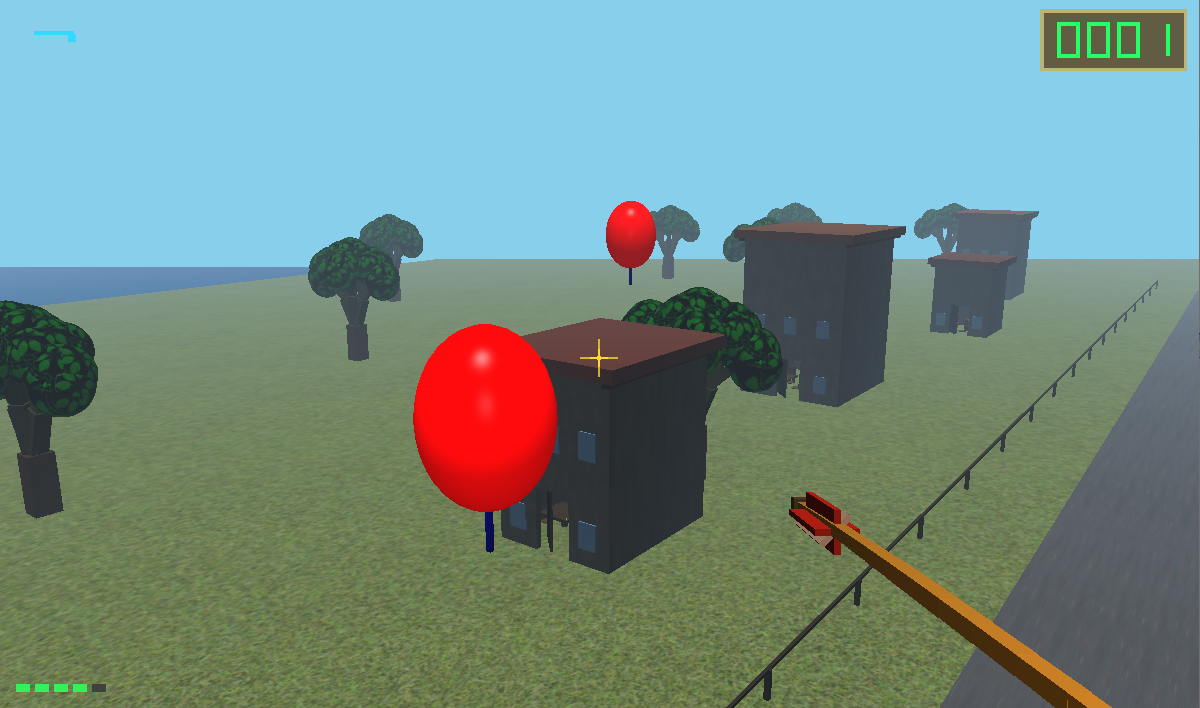
\includegraphics[width=0.92\textwidth]{image/scene_day.png}
    \caption{Full island environment in day mode --- ground, road, buildings, fractal trees, mountains, and clouds visible from a wide-angle camera position.}
    \label{fig:day}
\end{figure}

% ── 2. OBJECTIVES ────────────────────────────────────────────────────────────
\section{Objectives}

The primary objectives of this project are:

\begin{enumerate}[noitemsep]
    \item Develop a complete 3D interactive game using modern OpenGL (core profile, no deprecated fixed-function pipeline).
    \item Implement and compare the \textbf{Phong} and \textbf{Gouraud} illumination models with live run-time switching.
    \item Apply \textbf{texture mapping} using both GL\_REPLACE and GL\_MODULATE blending modes.
    \item Demonstrate \textbf{fractal recursive geometry} through procedurally generated trees.
    \item Construct a diverse 3D environment using only \textbf{primitive shapes} (cube, sphere, cone) composed via model matrix transformations.
    \item Implement \textbf{realistic projectile physics} including gravity, wind, and quaternion-based rotation.
    \item Render a \textbf{pixel-art HUD} (7-segment score display, combat interface, toast notifications) using orthographic projection.
    \item Provide an \textbf{automated demo tour} that showcases all rendering features within 90 seconds.
\end{enumerate}

% ── 3. TECHNOLOGIES ──────────────────────────────────────────────────────────
\section{Technologies and Libraries Used}

\begin{table}[h!]
\centering
\begin{tabular}{@{} l l @{}}
\toprule
\textbf{Technology} & \textbf{Role} \\
\midrule
OpenGL 3.3 Core & Primary 3D rendering API \\
GLFW            & Cross-platform window creation and input events \\
GLAD            & OpenGL extension/function loader \\
GLM             & Mathematics library: vectors, matrices, quaternions \\
stb\_image      & Single-header image loader for texture files \\
GLSL            & Vertex and fragment shader language \\
C++ (17+)       & Application logic, game state, data structures \\
\bottomrule
\end{tabular}
\caption{Libraries and their roles in the project.}
\end{table}

All rendering is done through \textbf{Vertex Array Objects (VAOs)}, \textbf{Vertex Buffer Objects (VBOs)}, and \textbf{Element Buffer Objects (EBOs)}. A single shared \texttt{cubeVAO} (24 vertices, 36 indices) is used for all cube-based objects. Sphere and Cone each have their own dedicated VAO generated procedurally at startup.

% ── 4. FEATURES ──────────────────────────────────────────────────────────────
\newpage
\section{Features Implemented}

% 4.1
\subsection{Geometric Primitives and Object Construction}

Every object in the scene is built from three basic geometric shapes:

\begin{itemize}[noitemsep]
    \item \textbf{Cube:} The most common primitive. Defined with 24 vertices (4 per face), 36 triangle indices, and per-vertex position, normal, and texture coordinate data. Stored once in a shared \texttt{cubeVAO} and reused for every box-shaped object.
    \item \textbf{Sphere:} Procedurally generated using spherical coordinates with 36 sectors and 18 stacks. Used for balloons, clouds, leaf clusters, the sun/moon, and the lighthouse lamp.
    \item \textbf{Cone:} Procedurally generated with 36 sectors, tapered sides, and a circular base cap. Used for decorative scene elements.
\end{itemize}

Each object is positioned and shaped by composing a model matrix from \textbf{translate $\rightarrow$ rotate $\rightarrow$ scale} operations. For example, a balloon body is simply a unit sphere scaled by $(0.6,\ 0.8,\ 0.6)$ to produce the characteristic oval shape.

A custom \texttt{rotate\_manual()} function implements \textbf{Rodrigues' rotation formula} for arbitrary-axis rotation without using \texttt{glm::rotate()}, satisfying the lab requirement:
\begin{equation}
    \mathbf{R}(\hat{u}, \theta) = \cos\theta\,\mathbf{I} + (1-\cos\theta)\,\hat{u}\hat{u}^T + \sin\theta\,[\hat{u}]_\times
\end{equation}

% 4.2
\subsection{Shading Models --- Phong vs.\ Gouraud}

Two complete GLSL shader pipelines are compiled at startup. Key~\texttt{8} switches between them instantly:

\begin{lstlisting}[language=C++]
// Shader selection at the start of every frame
Shader& lightingShader = vertexShaderMode ? gouraudShader : phongShader;
\end{lstlisting}

\textbf{Phong Shading (default):}
Lighting calculations are performed \emph{per fragment} inside the fragment shader. The surface normal is interpolated across the triangle and used to compute ambient, diffuse, and specular contributions at each pixel. This produces smooth, accurate highlights regardless of polygon count.

\textbf{Gouraud Shading:}
Lighting is computed \emph{per vertex} inside the vertex shader. The resulting color is then interpolated (Gouraud interpolation) across the triangle during rasterization. This is faster but produces visibly coarser specular highlights --- especially noticeable on large flat surfaces or low-polygon meshes. The difference between the two models is immediately apparent when viewing curved surfaces such as the balloon or the sphere-based clouds.

The Phong lighting equation computed per fragment is:
\begin{equation}
    \mathbf{I} = \mathbf{I}_a \cdot k_a + \mathbf{I}_d \cdot k_d (\hat{L}\cdot\hat{N}) + \mathbf{I}_s \cdot k_s (\hat{R}\cdot\hat{V})^n
\end{equation}
where $\hat{L}$ is the light direction, $\hat{N}$ is the surface normal, $\hat{R}$ is the reflection vector, $\hat{V}$ is the view direction, and $n$ is the shininess exponent.

% 4.3
\subsection{Lighting System and Day/Night Cycle}

Three types of light sources are combined to illuminate the scene:

\subsubsection*{Directional Light (Sun / Moon)}
A directional light with direction $(-0.2,\ -1.0,\ -0.3)$ illuminates the entire scene with parallel rays, simulating sunlight. At night (key \texttt{N}), its intensity drops to near zero and the color shifts to a cool blue to simulate moonlight:

\begin{table}[h!]
\centering
\begin{tabular}{@{} l l l @{}}
\toprule
\textbf{Component} & \textbf{Day Values} & \textbf{Night Values} \\
\midrule
Ambient  & (0.50, 0.50, 0.50) & (0.05, 0.05, 0.10) \\
Diffuse  & (0.80, 0.80, 0.80) & (0.10, 0.10, 0.10) \\
Specular & (1.00, 1.00, 1.00) & (0.10, 0.10, 0.10) \\
\bottomrule
\end{tabular}
\caption{Directional light values for day and night modes.}
\end{table}

\subsubsection*{Point Lights ($\times$2)}
Two point light sources are placed at the tower $(0,\ 5,\ 0)$ and near a tree $(15,\ 2,\ -15)$. They emit a warm amber glow and use the standard attenuation formula:
\begin{equation}
    F_{att} = \frac{1}{k_c + k_l \cdot d + k_q \cdot d^2}
\end{equation}
with constants $k_c=1.0$, $k_l=0.22$, $k_q=0.20$, giving an effective range of approximately 20 units. These lights turn \emph{on automatically} when night mode is activated and \emph{off automatically} during the day.

\subsubsection*{Spot Light (Flashlight)}
A spotlight is attached to the camera. It follows the player's view direction with a smooth cone edge defined by inner cutoff $12.5°$ and outer cutoff $15°$, using the GLSL \texttt{smoothstep} function for gradual falloff. Attenuation constants: $k_c=1.0$, $k_l=0.09$, $k_q=0.032$.

Each of the three Phong components (ambient, diffuse, specular) can be toggled independently with keys \texttt{5}, \texttt{6}, \texttt{7}, allowing isolated observation of each term's contribution.

\begin{figure}[H]
    \centering
    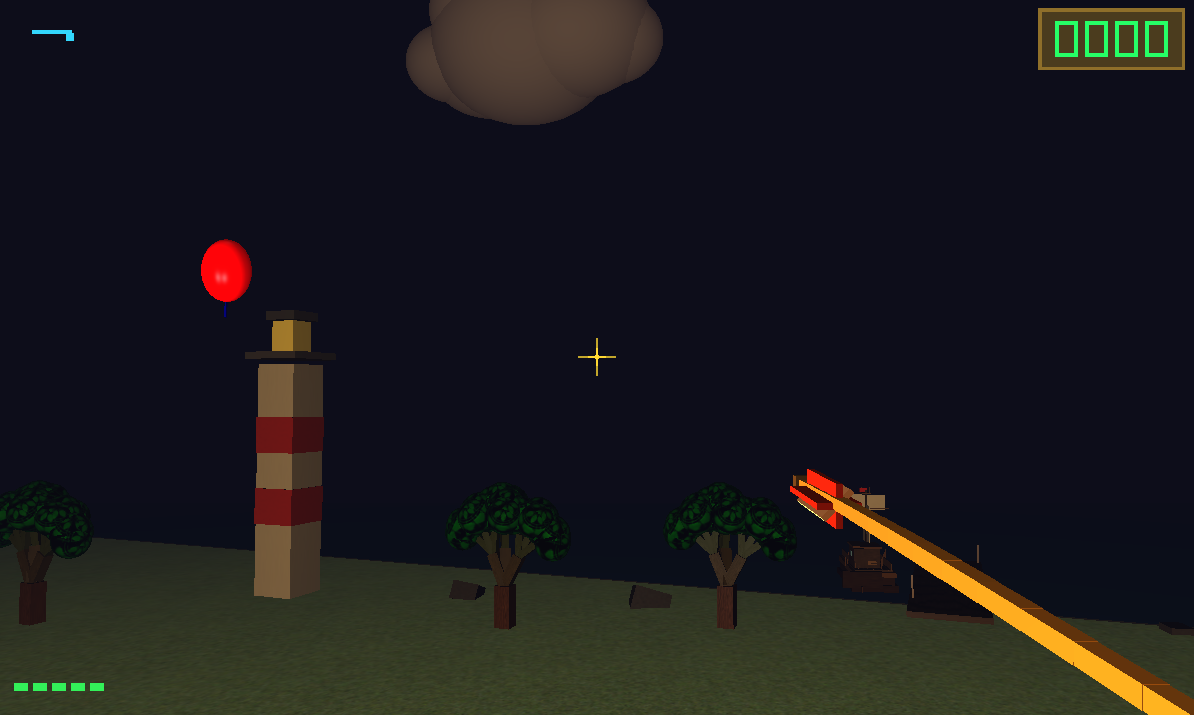
\includegraphics[width=0.92\textwidth]{image/scene_night.png}
    \caption{Night mode: directional light dimmed to moonlight, warm point lights active at the tower and tree locations, dark sky background.}
    \label{fig:night}
\end{figure}

% 4.4
\subsection{Texture Mapping}

Eight image textures are loaded using \texttt{stb\_image} at startup and applied to objects using two blending modes:

\begin{itemize}[noitemsep]
    \item \textbf{GL\_REPLACE:} The texture color completely replaces the base object color. Used where the texture itself defines the look (grass, asphalt).
    \item \textbf{GL\_MODULATE:} The texture color is multiplied with the lighting result, so shading and shadows still affect the surface. Used for all structural materials.
\end{itemize}

\begin{table}[h!]
\centering
\begin{tabular}{@{} l l l @{}}
\toprule
\textbf{Texture} & \textbf{Applied To} & \textbf{Mode} \\
\midrule
Grass    & Island ground              & GL\_REPLACE  (tiled 16$\times$) \\
Asphalt  & Road surface               & GL\_REPLACE  (tiled 9$\times$)  \\
Bark     & Tree trunks, pier, ship    & GL\_MODULATE \\
Bricks   & Tower, building walls      & GL\_MODULATE \\
Leaf     & Tree foliage spheres       & GL\_MODULATE \\
Rock     & Mountain faces             & GL\_MODULATE \\
Sail     & Ship sails                 & GL\_MODULATE \\
Concrete & Dock / pier surface        & GL\_MODULATE \\
\bottomrule
\end{tabular}
\caption{Textures, their targets, and blending modes.}
\end{table}

A \texttt{texScale} uniform is passed to the shader per object, allowing texture tiling to be proportional to the object's physical size (e.g., the large ground plane tiles at 16$\times$ to avoid stretching). All textures can be globally disabled with key \texttt{T} for before/after comparison.

% 4.5
\subsection{Procedural Balloon Shader}

Balloon surfaces are rendered using a \textbf{procedural fragment shader} rather than an image texture. The shader uses the dot product between the view direction and surface normal to generate a radial gradient:

\begin{lstlisting}[language=GLSL]
float rim = 1.0 - max(dot(norm, viewDir), 0.0);
vec3 balloonColor = mix(centerColor, edgeColor, pow(rim, 2.5));
\end{lstlisting}

This produces a glossy center-bright, edge-dark shading that simulates the look of an inflated latex balloon without any texture image.

% 4.6
\subsection{Fractal Tree Generation}

Trees are built using a \textbf{recursive fractal branching algorithm} implemented in \texttt{drawFractalTreeRec()}. The algorithm is inspired by the self-similar structure of real trees:

\begin{itemize}[noitemsep]
    \item \textbf{Recursion depth:} 4 levels.
    \item \textbf{Initial parameters:} length = 2.5 units, thickness = 0.8 units.
    \item \textbf{Per-level scaling:} Each child branch is scaled by 0.65$\times$ the parent's size.
    \item \textbf{Branching factor:} 3 children per node --- left (+25°), right ($-25$°), and straight ($\approx$5°). Each receives an additional small pseudo-random rotation based on its depth index for natural irregularity.
    \item \textbf{Branch primitive:} A cube scaled to (thickness, length, thickness) with bark texture applied.
    \item \textbf{Color interpolation:} Branches transition from brown at the base to green at higher levels, computed as a linear blend based on current depth.
    \item \textbf{Leaf clusters:} At terminal nodes (depth = 0), a green textured sphere (radius = 6$\times$ final thickness) replaces the branch to simulate a leaf mass.
\end{itemize}

Over 20 tree instances are placed across the island at varying positions.

% 4.7
\subsection{Weather System}

\subsubsection*{Rain Particles}
Pressing \texttt{F} activates the rain system. Up to \textbf{500 raindrop particles} are maintained in a pool. Each particle is a thin cube scaled $(0.02 \times 0.23 \times 0.02)$, rotated 14° on the X-axis to simulate wind-driven rain, and colored pale blue $(0.6,\ 0.7,\ 0.9)$. Each frame, active particles fall by \texttt{speed $\times$ dt}; when they reach ground level they reset to a random position above the scene. Only particles within 100 units of the camera are drawn.

\subsubsection*{Lightning / Thunder}
While rain is active, each frame has a 1/5000 probability of triggering a \textbf{lightning flash}. When triggered, the directional light's ambient and diffuse values spike to $(1.0,\ 1.0,\ 1.0)$ and the sky background flashes bright grey. The flash decays naturally over \textbf{0.12 seconds} as the timer counts down, then rain lighting values are restored.

\subsubsection*{Atmospheric Fog}
Exponential fog is applied in the fragment shader using the formula:
\begin{equation}
    \text{fogFactor} = e^{-\,\text{density} \times \text{fragDistance}}
\end{equation}
The final color is blended: $\mathbf{C}_{out} = (1 - \text{fogFactor})\,\mathbf{C}_{fog} + \text{fogFactor}\,\mathbf{C}_{lit}$. Fog density and color are set automatically: light haze during the day, denser dark-blue fog at night, and grey fog during rain.

% 4.8
\subsection{Combat System}

\subsubsection*{Bullet Mode}
Bullets travel in a straight line at 38 units/s. Each magazine holds 15 rounds with a 2-second reload. The first-person bullet model is composed of three aligned cubes: a brass casing $(0.025 \times 0.025 \times 0.12)$, a copper-colored pointed tip, and a grey primer cap. All three cubes share the same quaternion orientation derived from the projectile's velocity vector so they stay correctly aligned during flight.

\subsubsection*{Arrow Mode}
Arrows are affected by \textbf{gravity} (6 units/s²) and a random \textbf{wind force}, producing a parabolic arc. Each quiver holds 5 arrows with a 3-second reload. The arrow model uses a \textbf{14-segment Bézier-curved shaft}: control points are placed along a cubic Bézier curve and a cube segment is drawn at each interpolated position with thickness that varies slightly along the length. The arrowhead is formed by two perpendicular thin cubes (cross-blade shape), a gold collar ring, and three fletching feathers at the tail. The entire arrow rotates each frame to match its velocity direction using \textbf{quaternion slerp}:
\begin{lstlisting}[language=C++]
glm::quat targetRot = glm::rotation(glm::vec3(0,0,1),
                      glm::normalize(proj.velocity));
proj.rotation = glm::slerp(proj.rotation, targetRot, 0.35f);
\end{lstlisting}

\subsubsection*{Collision Detection}
A \textbf{3-point swept-sphere} check prevents fast projectiles from tunneling through thin targets: the system tests the previous frame position, the midpoint, and the current position against each balloon's bounding sphere. If any sample point is within the hit radius, a hit is registered.

% 4.9
\subsection{Balloon Enemy System}

Balloons spawn above the scene every 2 seconds at random $(x,z)$ positions and fall downward at varying speeds. Each balloon is stored as a struct:
\begin{lstlisting}[language=C++]
struct Balloon {
    glm::vec3 position, color;
    float scale, speed;
    bool active;
    float popTimer;
    std::vector<glm::vec3> fragments, fragVels;
};
\end{lstlisting}

On a successful hit, \texttt{popTimer} starts. The balloon's scale multiplier grows over 0.15~s (expansion animation) before the balloon is deactivated. Fragment cubes are then released with outward velocities to simulate an explosion. The game ends immediately when any balloon's y-position falls below the ground level.

% 4.10
\subsection{HUD (Heads-Up Display)}

All HUD elements are rendered using a dedicated flat-color shader with an \textbf{orthographic projection} in pixel space. Depth testing is disabled during HUD rendering so elements always appear on top of the 3D scene.

\subsubsection*{7-Segment Scoreboard}
The score (0--9999) is displayed as a 7-segment LED style readout in the top-right corner. Each digit is encoded as a 7-bit integer where each bit controls one segment (Top, Top-Left, Top-Right, Middle, Bottom-Left, Bottom-Right, Bottom). Segments are drawn as colored rectangles:
\begin{lstlisting}[language=C++]
static const int segs[10] = { 119,18,93,91,58,107,111,82,127,123 };
if (seg & 64) drawRect(color, 1.0f, dx, dy+halfH, digitW+t, t); // Top
if (seg & 32) drawRect(color, 1.0f, dx-halfW, dy+halfH*0.5f, t, halfH); // TL
// ... etc.
\end{lstlisting}
The display turns red when the game is over.

\subsubsection*{Combat HUD}
Shows current ammo (e.g.\ \texttt{12/15}), a reload progress bar, weapon mode indicator (bullet or arrow icon), and a static crosshair at the screen center.

\subsubsection*{Toast Notifications}
Short status messages appear centered at the bottom of the screen in a semi-transparent pill-shaped box. The dot-matrix font renderer uses a hand-coded 5$\times$7 pixel glyph table for each character. Text color varies by message type --- gold for shading/mode changes, cyan for lighting changes.

\begin{figure}[H]
    \centering
    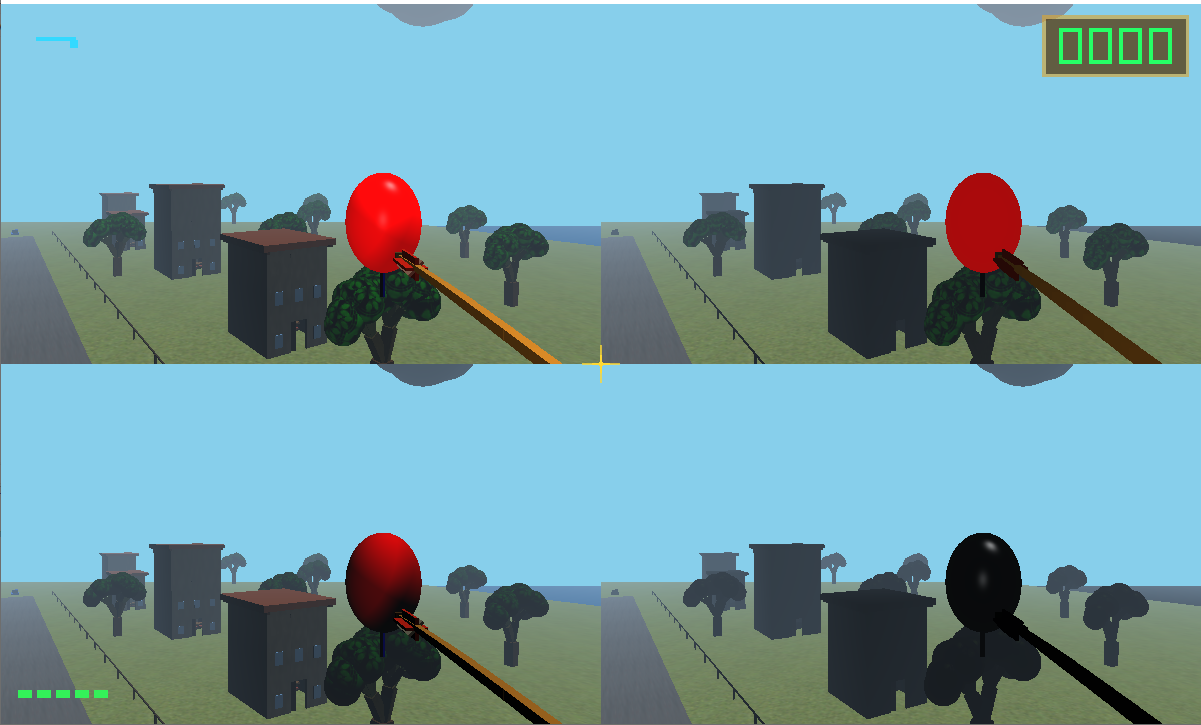
\includegraphics[width=0.92\textwidth]{image/split_viewport.png}
    \caption{Split viewport mode (key \texttt{V}): the screen is divided into four equal panes. Top-left shows the full combined render; top-right shows ambient only; bottom-left shows diffuse only; bottom-right shows specular only.}
    \label{fig:split}
\end{figure}

% 4.11
\subsection{Camera System and Automated Tour}

\subsubsection*{Fly Camera}
A custom \texttt{BasicCamera} class provides:
\begin{itemize}[noitemsep]
    \item \textbf{Fly-mode movement:} WASD for horizontal movement, Q/E for vertical.
    \item \textbf{Mouse look:} Yaw and pitch update from mouse delta; pitch is clamped to $\pm$89° to prevent gimbal lock.
    \item \textbf{Speed control:} Camera speed adjustable with \texttt{+}/\texttt{-} keys.
\end{itemize}

\subsubsection*{Automated Scenario Tour}
Pressing \texttt{0} starts a \textbf{90-second scripted demo tour}. Camera paths are computed using \textbf{Catmull-Rom spline interpolation} between 4 control points per scene, with an ease-in/out timing function $f(t) = t^2(3-2t)$ for smooth acceleration:

\begin{equation}
    \mathbf{P}(t) = \tfrac{1}{2}\bigl[(2\mathbf{P}_1) + (-\mathbf{P}_0+\mathbf{P}_2)t + (2\mathbf{P}_0-5\mathbf{P}_1+4\mathbf{P}_2-\mathbf{P}_3)t^2 + (-\mathbf{P}_0+3\mathbf{P}_1-3\mathbf{P}_2+\mathbf{P}_3)t^3\bigr]
\end{equation}

The tour sequence and timing:

\begin{table}[h!]
\centering
\begin{tabular}{@{} l l l @{}}
\toprule
\textbf{Time} & \textbf{Scene} & \textbf{Feature Shown} \\
\midrule
0--12 s  & Wide island fly-over    & Day mode, full environment \\
12--22 s & Tree \& lamp close-up  & Fractal trees, point light positions \\
22--32 s & Building walk-through  & Interior details; Night mode at 27 s \\
32--44 s & Night fly-over         & Phong → Gouraud → Phong shading switch \\
44--54 s & Night lighting         & Tower light off/on; Flashlight on/off \\
54--64 s & Wide shot              & Rain on/off; Lightning flash \\
64--70 s & Pull back              & Day mode restored \\
70--80 s & Close-up fly-over      & Textures off/on comparison \\
80--90 s & Steady orbit           & Ambient, Diffuse, Specular off/on \\
\bottomrule
\end{tabular}
\caption{Automated tour sequence (90 seconds total).}
\end{table}

\subsection{Split Viewport}

Pressing \texttt{V} divides the screen into four equal \textbf{viewports} using \texttt{glViewport()}. Each viewport renders the same scene with a different lighting configuration:
\begin{itemize}[noitemsep]
    \item \textbf{Top-Left:} All components active (full Phong render).
    \item \textbf{Top-Right:} Ambient component only --- shows the base color floor.
    \item \textbf{Bottom-Left:} Diffuse component only --- shows shading from light direction.
    \item \textbf{Bottom-Right:} Specular component only --- highlights surfaces facing the light.
\end{itemize}

% ── 5. SCENE OBJECTS ─────────────────────────────────────────────────────────
\newpage
\section{Scene Objects and Environment}

The entire island environment is built from the three geometric primitives described in Section~4.1. No external 3D models are used --- every object is assembled by composing and transforming primitive shapes.

\begin{table}[h!]
\centering
\renewcommand{\arraystretch}{1.2}
\begin{tabular}{@{} p{3.5cm} p{9cm} @{}}
\toprule
\textbf{Object} & \textbf{Construction Notes} \\
\midrule
Island / Ground  & Single cube scaled (150$\times$1$\times$180); grass texture tiled 16$\times$. \\
Ocean Water      & Four large flat cubes (e.g.\ $500\times0.5\times160$) in dark blue-grey surrounding the island. \\
Sandy Beach      & Thin cubes in tan color along each island edge. \\
Road             & Flat cube (8$\times$0.1$\times$90); asphalt texture. \\
Fence            & Vertical post cubes with horizontal rope cubes connecting them. \\
Defense Tower    & Shaft cube (2$\times$8$\times$2, brick texture) + platform (4$\times$0.2$\times$4) + 4 railing posts. \\
Balloons         & Oval sphere (0.6$\times$0.8$\times$0.6) + string cube; procedural shader. \\
Fractal Trees    & Recursive bark-textured cubes (depth 4) + leaf spheres; 20+ instances. \\
Buildings        & Multi-cube shell (walls, roof, door rotated $-45°$, windows) + interior (bar counter, stools, table, chairs, shelves, bottles, ceiling lantern). \\
Mountains        & 7 rotated/scaled cubes per mountain; colors blended 40\% toward sky blue for atmospheric depth haze; snowcap on central peak. \\
Clouds           & 8 overlapping spheres per cloud, off-white color; 10 instances scattered across sky. \\
Sailing Ship     & Hull (inner + outer + keel cubes) + deck planks + waterline stripe + mast (5 units tall) + sail (textured) + cabin with windows + anchor chain. \\
Dock / Pier      & Plank cubes + support pillar cubes extending into water. \\
Lighthouse       & Striped cube stack + sphere lamp at top. \\
Sun / Moon       & Single sphere (radius 5); yellow for day, cool white for night. \\
Rain             & 500 thin tilted cubes (0.02$\times$0.23$\times$0.02), per-frame particle update. \\
\bottomrule
\end{tabular}
\caption{Scene objects and their construction approaches.}
\end{table}

% ── 6. CONTROLS ──────────────────────────────────────────────────────────────
\newpage
\section{Controls}

\begin{table}[h!]
\centering
\begin{tabular}{@{} l l @{}}
\toprule
\textbf{Key / Input} & \textbf{Action} \\
\midrule
W / A / S / D        & Move camera (fly mode) \\
Q / E                & Move up / down \\
Mouse (drag)         & Look around (yaw and pitch) \\
M                    & Toggle mouse lock \\
Space / Right-Click  & Shoot (current weapon) \\
Ctrl + M             & Switch bullet $\leftrightarrow$ arrow mode \\
N                    & Toggle day / night mode \\
F                    & Toggle rain \\
1                    & Toggle directional light \\
2                    & Toggle point lights \\
3                    & Toggle spot light (flashlight) \\
4                    & Freeze / unfreeze balloons \\
5 / 6 / 7            & Toggle ambient / diffuse / specular \\
8                    & Switch Phong $\leftrightarrow$ Gouraud shading \\
T                    & Toggle all textures \\
V                    & Toggle split viewport (4 panes) \\
0                    & Start / stop automated 90 s scenario tour \\
R                    & Restart game after game over \\
\bottomrule
\end{tabular}
\caption{Complete keyboard and mouse controls.}
\end{table}

% ── 7. CODE ARCHITECTURE ─────────────────────────────────────────────────────
\section{Code Architecture}

\begin{table}[h!]
\centering
\begin{tabular}{@{} l p{9cm} @{}}
\toprule
\textbf{File} & \textbf{Description} \\
\midrule
\texttt{main.cpp}              & Main application entry point; game loop, all rendering functions, input callback, game-state logic, HUD drawing, scenario tour. \\
\texttt{shader.h}              & Shader class: compile, link, and uniform setter helpers. \\
\texttt{basic\_camera.h}       & Fly-mode camera with WASD movement and mouse look. \\
\texttt{sphere.h}              & Parametric sphere generator (sectors $\times$ stacks). \\
\texttt{cone.h}                & Parametric cone generator with base cap. \\
\texttt{pointLight.h}          & Point light data struct with toggle methods. \\
\texttt{DirectionalLight.h}    & Directional light data struct with toggle methods. \\
\texttt{SpotLight.h}           & Spot light struct with cutoff and attenuation. \\
\texttt{stb\_image.h}          & Single-header image loading library. \\
\midrule
\texttt{*ForPhongShading.vs/.fs}   & Per-fragment Phong lighting pipeline. \\
\texttt{*ForGouraudShading.vs/.fs} & Per-vertex Gouraud lighting pipeline. \\
\texttt{vertexShader.vs/.fs}       & Flat-color shader used for HUD rendering. \\
\texttt{colorShader.vs/.fs}        & Simple color-only shader. \\
\bottomrule
\end{tabular}
\caption{Source files and their responsibilities.}
\end{table}

% ── 8. CONCLUSION ────────────────────────────────────────────────────────────
\newpage
\section{Conclusion}

Balloon Shooter 3D is a feature-complete 3D application that demonstrates a wide spectrum of computer graphics techniques within a single real-time OpenGL project. Starting from raw GLSL shaders and geometric primitives, the project builds an entire playable world --- islands, buildings, fractal trees, weather, and ocean --- without relying on any external model files or rendering frameworks beyond OpenGL itself.

The dual shading pipeline (Phong and Gouraud) with live switching gives an immediate visual understanding of how per-fragment vs.\ per-vertex lighting affects surface quality. The dynamic lighting system, with its three light types and independently controllable Phong components, provides an in-depth hands-on exploration of the illumination model. The weather system, projectile physics, and fractal geometry further extend the project beyond a basic rendering demo into a genuinely interactive experience.

The 90-second automated tour distills all rendering features into a time-boxed presentation sequence with smooth camera motion, making it easy to demonstrate the project in a lab setting without manual navigation. Overall, the project fulfills and extends the requirements of the CSE~4208 Computer Graphics Laboratory.

\end{document}
